\section*{Autres informations}
\label{sec:autres}
\addcontentsline{toc}{section}{Autres informations}

\subsection*{Liens utiles}
\label{subsec:liens}
\addcontentsline{toc}{subsection}{Liens utiles}
Pour ceux qui sont intéressés par le domaine de la finance ou qui cherchent à étendre leurs champs d'expertise, la désignation professionnelle CFA peut être une très bonne option. C'est sans doute la désignation du monde de la finance qui est la plus reconnue à l'international et un nombre considérable d'actuaires la possèdent. Afin d'obtenir cette désignation, l'on doit passer trois examens (\emph{Level I, II} et \emph{Level III}) et avoir quatre ans d'expérience pertinente dans le milieu de la finance. Concernant l'expérience demandée, il est difficile de connaître les critères exactes du CFA Institute mais, généralement, il faut qu'une majorité du temps de travail de ces quatre années soit relié à la gestion d'actifs au sens large. Les examens \emph{Level II \emph{et} Level III} sont offerts seulement une fois par année, le premier samedi du mois de juin, alors que le \emph{Level I} est également offert au mois de décembre. Pour plus d'informations, consulter la page du \href{https://www.cfainstitute.org/Pages/index.aspx}{\emph{CFA Institute}}. Vous pouvez également lire l'article \href{http://blog.coachingactuaries.com/why-would-actuaries-consider-getting-a-cfa/}{\emph{Why would Actuaries consider getting a CFA?}}.\vspace{\baselineskip}

%%% TODO: faire des sections qui décrivent les examens CFA? De plus en plus de gens qui s'intéressent au titre...

Ceux qui sont intéressés par l'informatique et le \emph{data science} pourront s'informer au sujet de la création du \href{http://www.casact.org/press/index.cfm?fa=viewArticle&articleID=3083}{CAS Institute}.\vspace{\baselineskip} 


\newpage
\subsection*{Changements aux prérequis pour devenir Associé}
\label{subsec:changeasa}
\addcontentsline{toc}{subsection}{Changements aux prérequis pour devenir Associé}
\subsubsection*{SOA}
La SOA a amorcé en 2017 un important processus de restructuration des prérequis pour devenir Associé. La nouvelle structure est effective à partir du $1^{er}$ juillet 2018. Le plus gros changement est l’ajout de deux nouveaux examens (SRM et PA), mais ce sont quasi toutes les composantes qui sont modifiées d'une manière ou d'une autre. Ces changements au curriculum sont guidés par deux facteurs clés:

\begin{itemize}
\item L'ajout de l'analyse prédictive aux connaissances jugées essentielles pour devenir Associé;
\item Un meilleur équilibre entre les notions d'assurance court terme et long terme.
\end{itemize}
 Les changements subis par chaque composante sont mentionnés dans la section qui lui correspond.

\subsubsection*{CAS}
De son côté, la CAS a aussi amorcé un processus de restructuration pour 2018, mais les changements sont moins drastiques que pour la SOA. En pratique, l'ancien examen S devient l'examen MAS-I, et l'ancien examen C devient l'examen MAS-II. Également, la CAS a annoncé qu’elle reconnaîtrait les nouveaux formats des examens FM/2 et IFM/3F instaurés par la SOA. \textit{Les changements seront traités plus en détail dans les sections correspondantes du document dans une prochaine version de celui-ci.}

\vspace{\baselineskip} 

Quelques liens supplémentaires :
\begin{enumerate}
\item \href{https://www.soa.org/Education/General-Info/2016-asa-cera-curriculum-changes.aspx}{Annonce du 28 juin par la SOA}
\item \href{https://soa.qualtrics.com/CP/File.php?F=F_0TDd9bj143TrCW9}{Annonce préliminaire de la SOA (janvier 2016)}
\item \href{https://www.soa.org/Education/General-Info/2016-transition-rules-asa-candidated.aspx}{L’équivalence des examens actuels dans le système à venir}
\item \href{http://www.casact.org/press/index.cfm?fa=viewArticle&articleID=3273}{Annonce de la CAS pour le nouveau format de FM/2 et MFE/3F}
\end{enumerate}
\vspace{\baselineskip} 

Les diagrammes ci-dessous vous permettent d'observer d'une manière graphique les changements apportés aux prérequis pour devenir Associé, tant du côté de la SOA que de celui de la CAS.

\begin{figure}[hp]
\begin{center}
\textbf{Changements aux prérequis pour devenir Associé (SOA)}\par\medskip
\end{center}
\hfill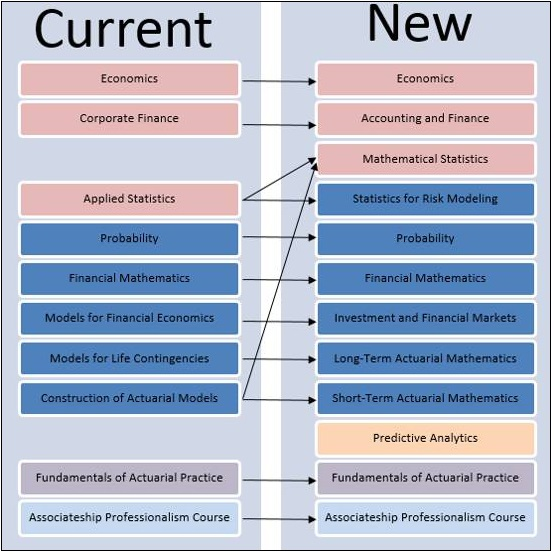
\includegraphics[scale=0.8]{Change_ASA.PNG}\hspace*{\fill}
\caption{Équivalences des examens actuels dans le système à venir (SOA)}
\end{figure}
\par
\begin{figure}[hp]
\begin{center}
\textbf{Changements aux prérequis pour devenir Associé (CAS)}\par\medskip
\end{center}
\hfill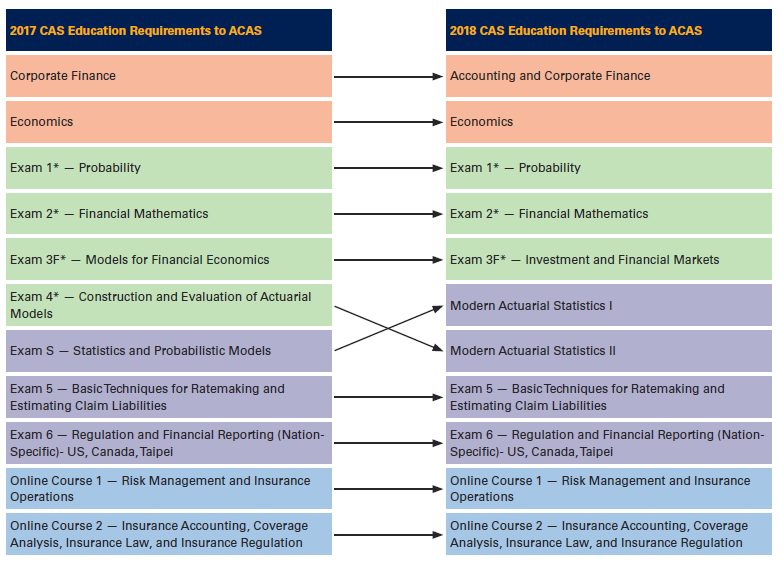
\includegraphics[scale=0.6]{Change_ASA_CAS.PNG}\hspace*{\fill}
\caption{Équivalences des examens actuels dans le système à venir (CAS)}
\end{figure}
\par

\newpage